
A basic fact to obtain this parametrization is the following.

\begin{figure}
    \centering
    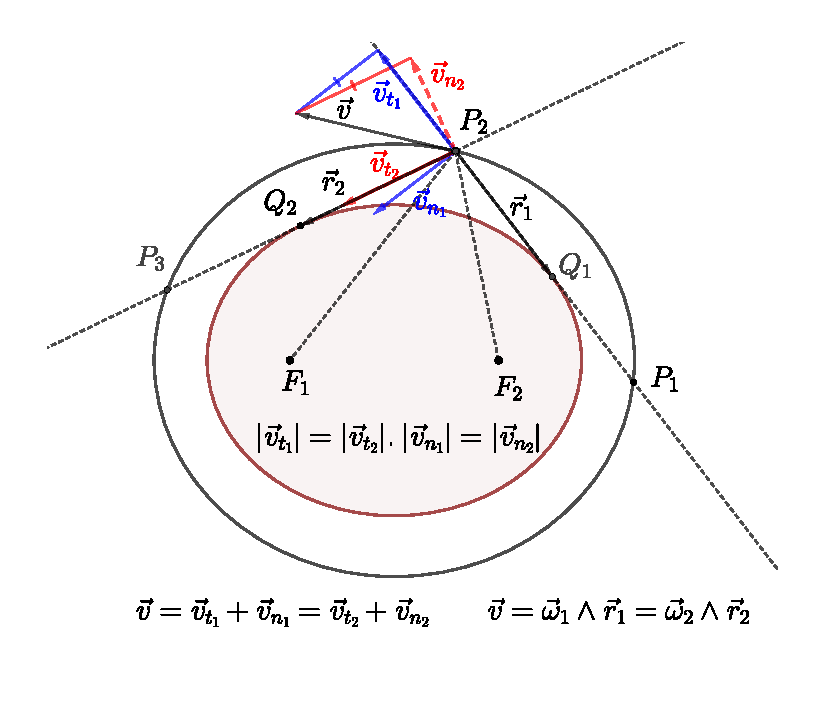
\includegraphics[width=\textwidth]{pics_02_040_param_jacobi.pdf}
    \caption{ Angular velocity $\vec v=\vec \omega\wedge \vec r$. } 
    \end{figure}
Referring to \cref{fig:02-velocidade-angular}:

\begin{proposition} 
Consider a 3-periodic segment $P_1P_2$ and $P_2P_3$  and contact points $Q_1$ and $Q_2$ with the caustic in an elliptic billiard. Let $\vec v$ the vector velocity of $P_2(t)$. Let $\vec r_1=Q_1-P_2$ and $\vec r_2=Q_2-P_2$. Then
\[ |\vec \omega_1|\;|\vec r_1|=|\vec \omega_2|\; |\vec r_2|\]
where $\vec v=\vec\omega_1\wedge r_1= \vec\omega_2\wedge \vec r_2$.

\label{fig:02-velocidade-angular}
\end{proposition}

\begin{proof} Let $\vec v=P_2'(t)$. From Graves's theorem, $|\vec r_1|+|\vec r_2|-\text{arc}(Q_1,Q_2)=\text{cte}$,  and therefore it follows that in decomposition of $\vec v=\vec v_{t_1}+\vec v_{n_1}=\vec v_{t_2}+\vec v_{n_2}$ we have that $|\vec v_{t_1}|=|\vec v_{t_2}|$ and  $|\vec v_{n_1}|=|\vec v_{n_2}|$. The result follows from the   definition of angular velocity. More details see \cite{stachel2021-billiards-param}.
\end{proof}
 
\textcolor{red}{ronaldo}
 
Since in this chapter we are considering billiard 3-periodics, so above $N=3$, and $\tau=1$. As shown in \cref{fig:02-jacobi-param}, under the Jacobi parametrization each of the 3 vertices of billiard 3-periodics follows the exact same curve, albeit with a 120-degree phase.

Recall the sum of cosines is constant for billiard 3-periodics. \cref{fig:02-jacobi-cos-param} shows how individual cosines follow either (i) 3-distinct curves, or (ii) the same exact curve (at different phases) if the parametrization is standard or Jacobi, respectively.

\begin{figure}
    \centering
    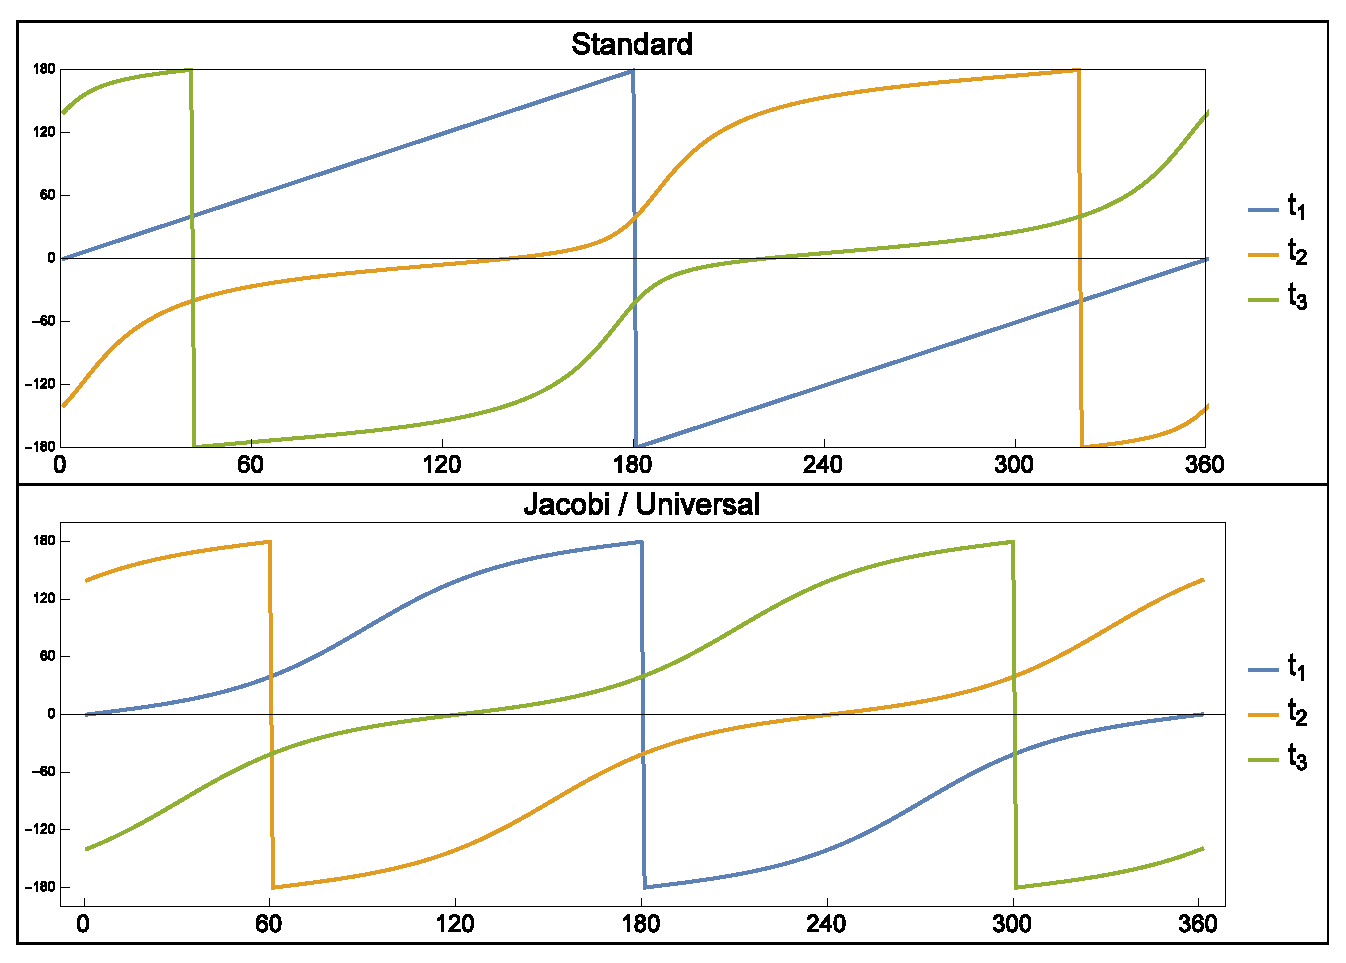
\includegraphics[width=\textwidth]{pics_02_050_parametrizations}
    \caption{The ``position'' $\theta_i$ (vertical axis) of a point on an ellipse with semi-axes $a,b$ vs the billiard 3-periodic parameter (horizontal axis). \textbf{Top:} vertex  under ``standard parametrization'', i.e., $P_1(t)=[a\cos{t},b\sin{t}]$. Notice while $P_1$'s position evolves linearly, those of $P_2$ and $P_3$ are different curves. \textbf{Bottom:} Said positions under Jacobi's parametrization. Notice the three positions are 120-degree delayed copies of one another.}. 
    \label{fig:02-jacobi-param}
\end{figure}

\begin{proof}
\textcolor{red}{ronaldo}
\end{proof}
\begin{figure}
    \centering
    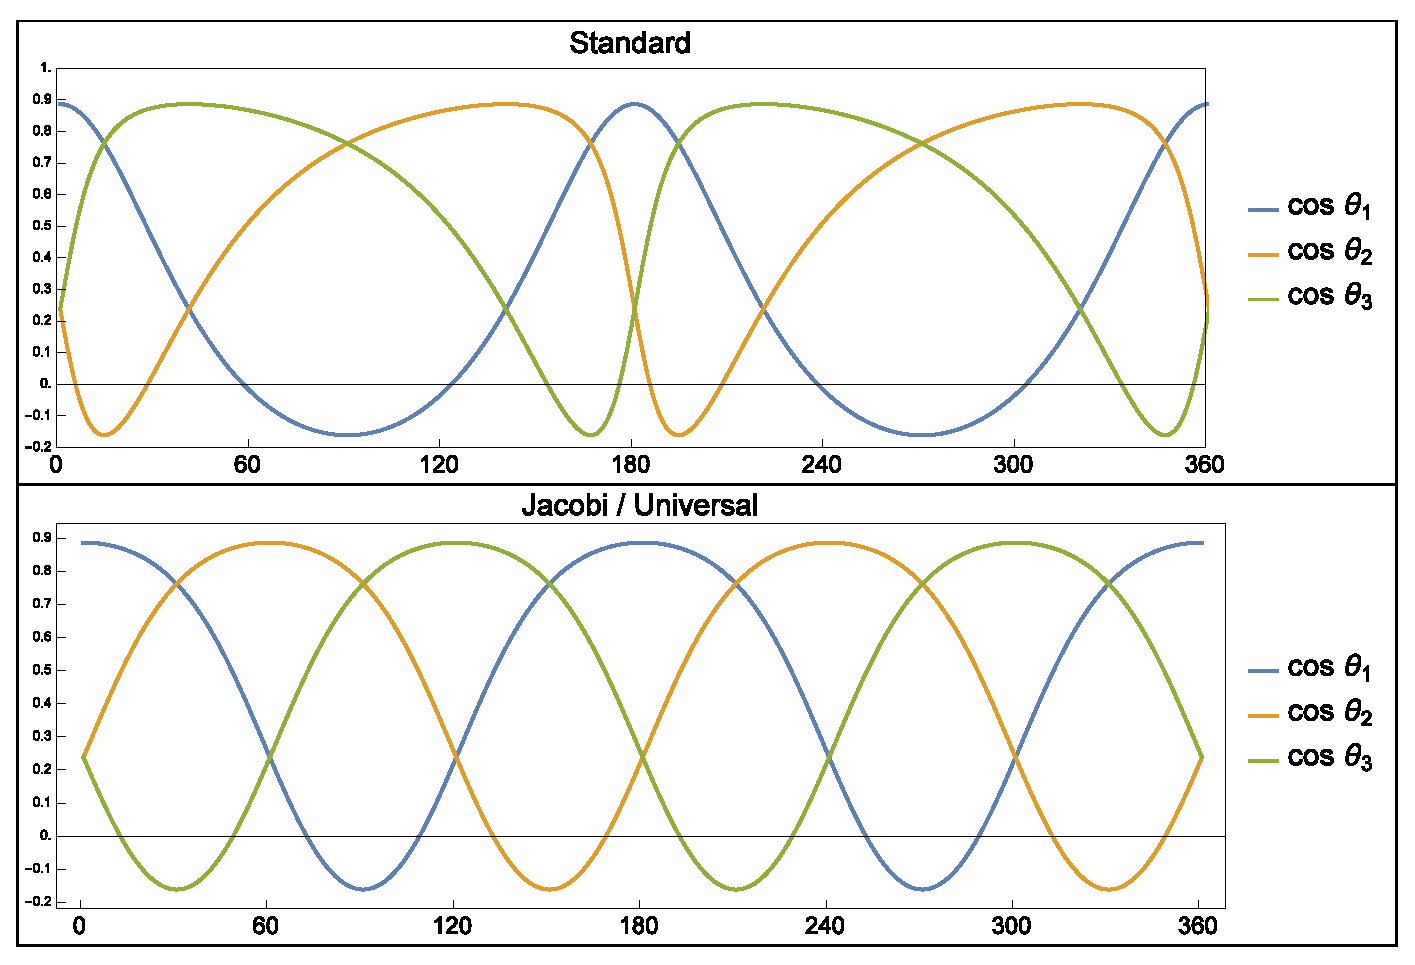
\includegraphics[width=\textwidth]{pics_02_060_cos_parametrizations}
    \caption{The cosines $\cos(theta_i)$ of billiard 3-periodic internal angles for the standard (top) and Jacobi parametrizations (bottom). While in the former case the three curves are distinct, in the latter case all cosines follow the same curve at different phases.}
    \label{fig:02-jacobi-cos-param}
\end{figure}